\documentclass{article}

\usepackage{mathtools,amssymb}
\usepackage{enumerate}
\usepackage{fancyvrb}
\usepackage{fullpage}
\usepackage{graphicx}


\title{Intermediate Test 5}
\author{Stellenbosch Camp 2019}
\date{Time: $4$ hours}

\begin{document}
\maketitle
\thispagestyle{empty}

\hfill\textit{Each question is worth 7 marks.}

\vfill
\vfill


\begin{enumerate}[1.]

\item % Emile, C
Given the below colouring, is it possible to invert the colours of rows or the colours of columns in some order to achieve a completely white board?
\begin{center}
    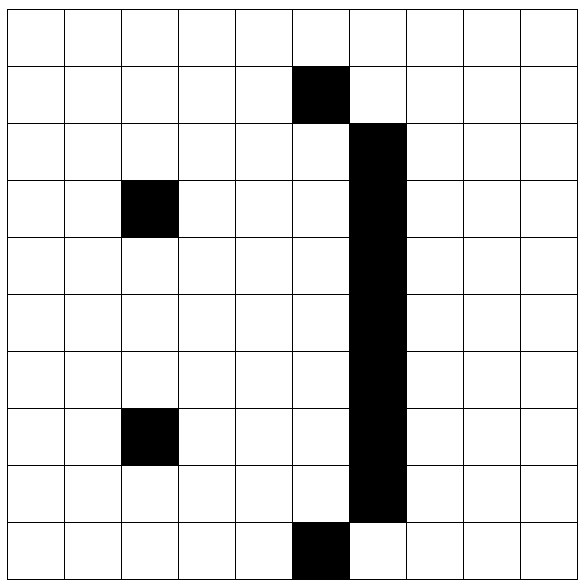
\includegraphics[width=0.5\textwidth]{test_5_q_1.png}
\end{center}

\vfill

\item % , 2018 December Monthly Assignment Q1
Let $n$ be a positive integer greater than 2. Let $r_1$ be the smallest odd divisor of $n$ greater than $1$ and let $r_2$ be the largest odd divisor of $n$. Find all $n$ such that
\begin{center}
 $n=5r_{1}+3r_{2}$
\end{center}

\vfill

\item % 2001 booklet, The Monthly Problem Sets number 4
For each positive integer $k$, define the sequence $(a_{n})$ by
\begin{align*}
	a_{0} &= 1 \\
	a_{n} &= kn + (-1)^{n}a_{n-1} \quad \text{for each } n \geqslant 1.
\end{align*}
Determine all values of $k$ for which 2000 is a term of the sequence.


\vfill

\item % Moldova 2018, 7.8, G
Let $\triangle XYZ$ be such that $\angle XZY = 30^o$. Let $M$ be a point inside $\triangle XYZ$. Let $A$ and $B$ be points on $XZ$ and $YZ$ respectively such that $\angle ZAM = \angle ZBM = 90^o$. Prove that $ZM = 2 \cdot AB$.

\vfill

\item % The Malwande, A
\newcommand{\QQ}{\mathbb{Q}}
Find all functions $f : \QQ \to \QQ$ such that
\[ f(x^2) +f(x+2y) = (x+1)f(x) +2f(y) \]
for all $x, y \in \QQ$. 


\vfill

\item % Austrian MO Q15, C
In the country of Oddland, there are stamps with values $1$ cent, $3$ cents, $5$ cents, etc., one type for each odd number.
the rules of Oddland Postal Services stipulate the following: for any two distinct values, the number of stamps of the higher value on an envelope must never exceed the number of stamps of the lower value.

In the country of Squareland, on the other hand, there are stamps with values $1$ cent, $4$ cents, $9$ cents, etc., one type for each square number.
Stamps can be combined in all possible ways in Squareland without additional rules.

Prove that for every positive integer $n$:
In Oddland and Squareland there are equally many ways to correctly place stamps of a total value $n$ cents on an envelope.
Rearranging the stamps on an envelope makes no difference.


\end{enumerate}


\vfill
\vfill

% ASCII art
\begin{center}
\begin{BVerbatim}
  __       __
  \ `-'"'-` /
  / \_   _/ \
  |  d\_/b  |
 .'\   V   /'.
/   '-...-'   \
| /         \ |
\/\         /\/
==(||)---(||)==
\end{BVerbatim}
\end{center}

\end{document}
